
\section{Website}

\begin{figure}[h]
	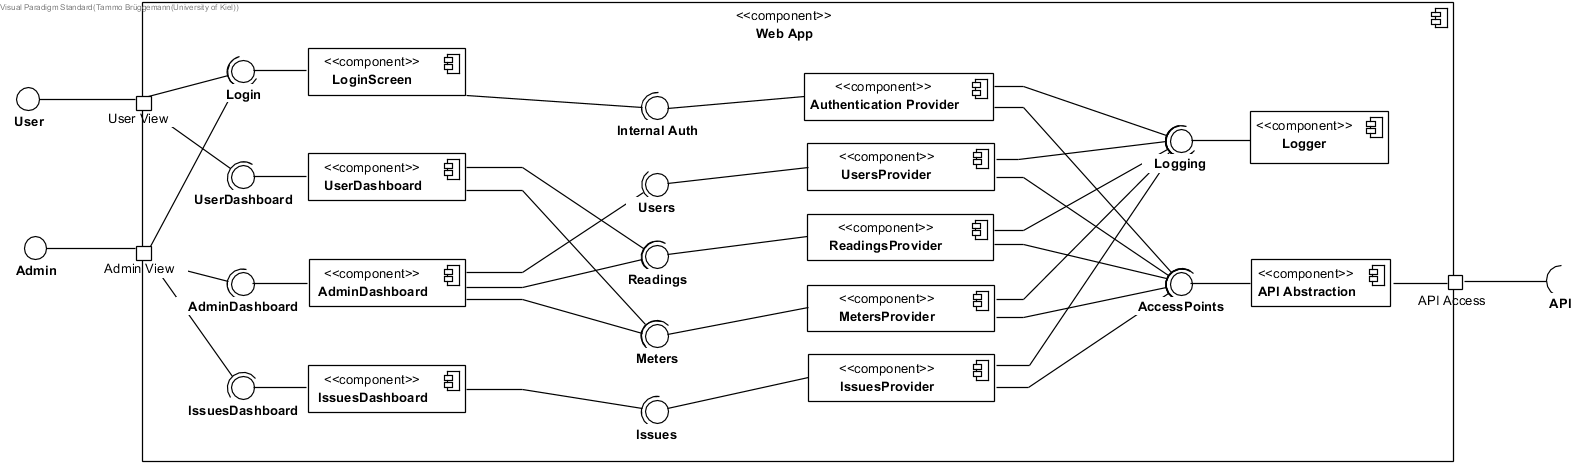
\includegraphics[scale = 0.45]{./img/Diagrams/Website-Components} 	
	\caption{Komponentendiagramm - Website} 
\end{figure}

In der Architektur der Web-Application kann man grob in 3 Spalten unterteilen. 
\\ \\
Wobei die rechte Spalte die Service Ebene darstellt, hier befindet sich eine API Abstraction. Die API Abstraction abstrahiert alle REST-Endpunkte welche wir in der Web-Applikation benötigen. Außerdem liegt hier ein Logger, welcher uns im Entwicklungsprozess Fehlermeldungen und Logpunkte auf der Console ausgibt. Optional könnte man diese auch an einen Logservice(z.B.: Sentry) schicken.
\\ \\
In der mittleren Spalte befinden sich alle Provider. Diese stellen der Benutzeroberfläche globale Informationen (state) zur Verfügung. Hier werden API Anfragen (vom Service abstrahiert) getriggert und die entsprechenden Daten gesammelt und gecached.
\\ \\
In der linken Spalte liegen die Benutzeroberflächen, worauf die Benutzer und Administratoren zugreifen. Diese benutzen die Provider, um Informationen von der API zu erhalten.

\newpage

\section{App}

\begin{figure}[h]
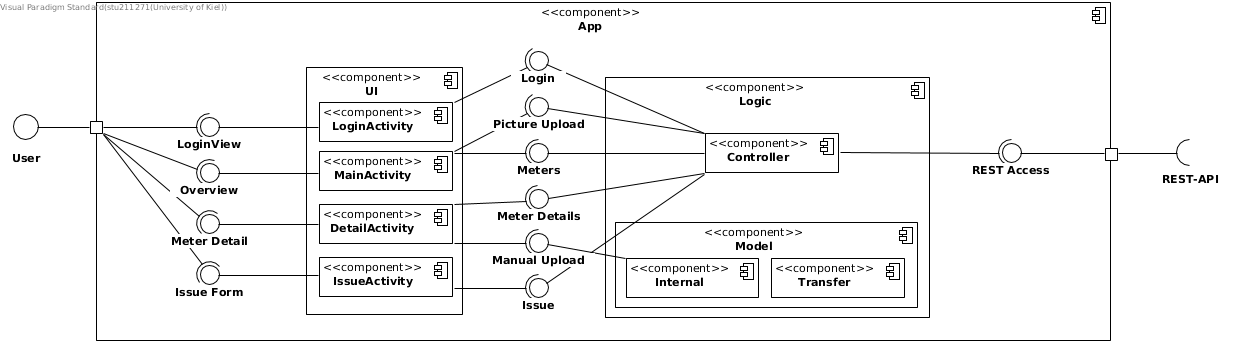
\includegraphics[scale=0.45]{img/diagrams/AppComponentDiagram}\caption{Komponentendiagramm - App}  
\end{figure}

Die App ist in mehrere Komponenten aufgeteilt, von denen die meisten direkt die Java-Packages des Projektes darstellen. Ausnahmen sind die Actvities in der UI Komponente, die wir hier eintragen obwohl sie häufig nur eine Activity-Klasse umfassen, weil sie darüber hinaus mehrere XML Dateien und andere Resourcen nutzen.\\
Die meisten Anfragen der UI gehen an die Controller Klassen, die außerdem als Fassade zwischen Front- und Backend der App dienen. Allerdings Kommuniziert die UI bei manuellen Uploads direkt mit der Meter Klasse, die in der Internal Komponente liegt.\\ \\
Die Transfer Komponente enthält alle DTOs des Projekts, und stellt paging support bereit, der von der Meter Klasse in Internal benutzt wird.\\
Internal enthält Datenobjekte, die die DTOs für den Rest der Anwendung abstrahieren.

\section{Back-End}

\begin{figure}[h]
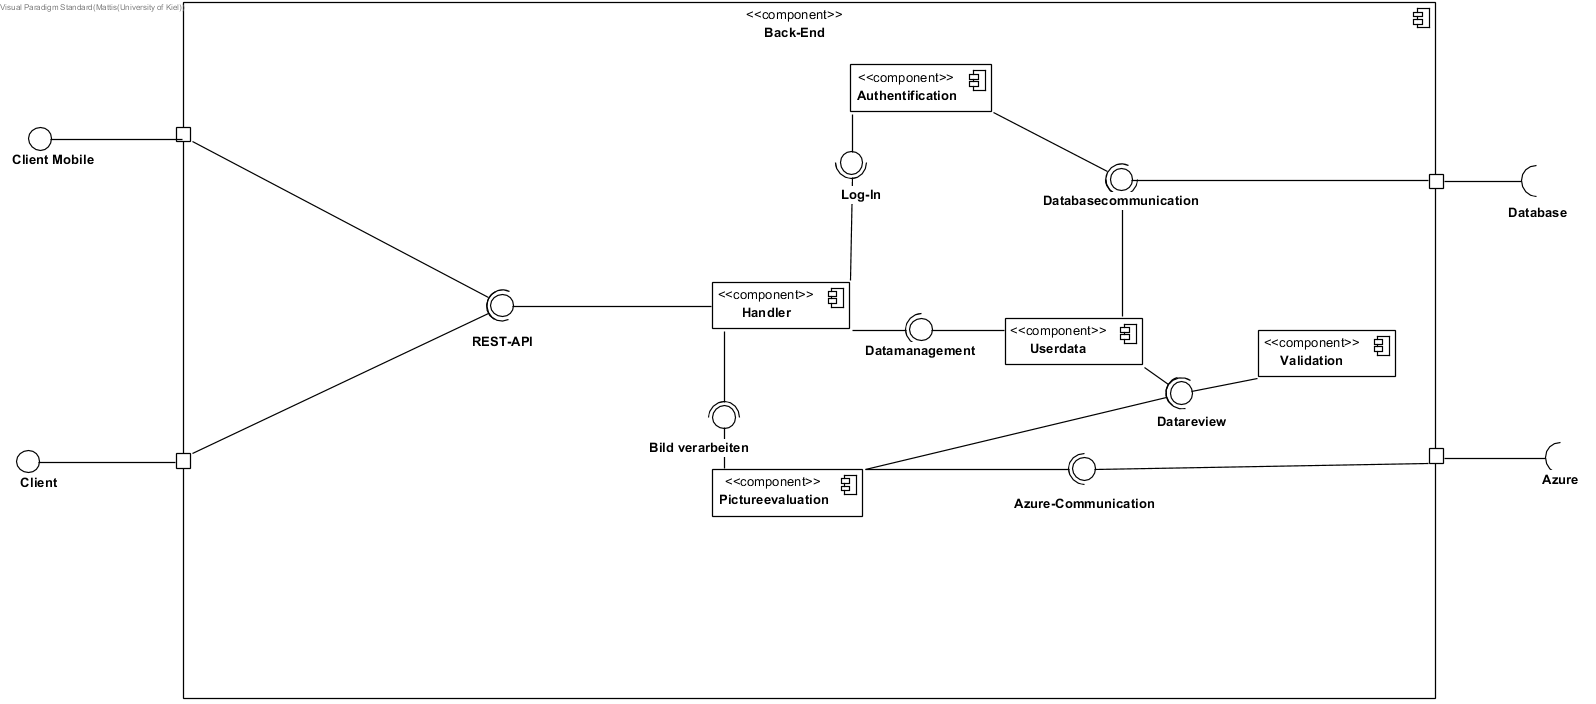
\includegraphics[width=15cm]{img/diagrams/component-back-end}
\caption{Komponentendiagramm - Back-End} 
\end{figure}

Zusammengesetzt ist das ''Back-End'' aus mehreren Komponenten und Schnittstellen, die untereinander interagieren.\\
Dabei regelt die ''Handler''-Komponente den Dateneingang durch Nutzeranfragen, indem sie die Daten an die für sie zuständigen Subkomponenten weiterleitet. Dies geschieht über die von diesen Komponenten angebotenen Schnittstellen. Die Nutzeranfragen aus App und Browser werden dabei durch die ''REST-API''-Schnittstelle angenommen, welche von der ''Handler''-Komponente zur Verfügung gestellt wird.\\
Um zu überprüfen ob Nutzer privilegiert sind bestimmte Anfragen zu stellen existiert die ''Authentification''-Komponente. Diese verhindert damit, dass Nutzer Operationen durchführen, zu welchen sie nicht befugt sind. Zu diesem Zweck stellt sie dem ''Handler'' eine ''Verify''-Schnittstelle zur Verfügung. Um die Befugnis eines Benutzers für eine bestimmte Operation zu überprüfen, benutzt die ''Authentifikation'' die ''Database-Communication''-Schnittstelle. Über diese werden die benötigten Rechte mit den in der Datenbank gespeicherten Rechten des Benutzers abgeglichen.\\
Weiterhin wird diese ''Data-Communication''-Schnittstelle von der ''User-Data''-Komponente genutzt. ''User-Data'' ermöglicht bei entsprechenden Privilegien das Abrufen oder Ändern von Kundendaten. Diese Komponente wird insbesondere genutzt um Zählerstände zu aktualisieren.\\
Die gewünschten Zugriffe auf Kundendaten erfolgen über die von der ''User-Data''-Komponente bereitgestellte ''Data-Management''-Schnittstelle, welche von der ''Handler''-Komponente verwendet wird.\\
Bei Veränderungen der Daten in ''User-Data'' werden diese durch die ''Datareview''-Schnittstelle an die ''Validation''-Komponente weitergeleitet. Dort werden Zählerstände und Nummern auf ihr Format, sowie Passwörter auf Sicherheitsstandards überprüft.\\
Auf die ''Data-Review''-Schnittstelle greift ebenfalls die ''Picture-Evaluator''-Komponente zu, um Zählernummern und Zählerstände auf Validität zu überprüfen. Diese Werte erhält die Komponenente von der ''adesso-Picture-Recognition'', welche die Bilder extern auswertet. Verbunden sind diese dabei über die ''Picture-Evaluation''-Schnittstelle. Die Bilder welche ausgewertet werden sollen gelangen über die ''Picture-Handling''-Schnittstelle, welche von der ''Picture-Evaluator''-Komponente angeboten wird, in eben diese. Umgekehrt werden die daraus erhaltenen Daten über die gleiche Schnittstelle an die ''Handler''-Komponente zurückgesendet. Die ''Picture-Evaluator''-Komponente fungiert somit als Knotenpunkt für die Bildverarbeitung. 

